% !TEX program = xelatex
% AI-effects 프로젝트 --- 점유율 지표 A·B·C와 노출도 3개의 순위 비교 엑셀 파일 설명.
% 표 본문: results/table/35_spearman.tex, 35_cross.tex, 35_cross_rev.tex, 35_topC10.tex, 35_notes.tex
%          (code/04_18_analysis_kor_share_exposure_rank.do가 생성)
% 설명 대상: results/table/35_kor_share_exposure_rank.xlsx
% 관련: paper 23(노출도의 KSCO 변환), 27(점유율 지표 A~D), 28(점유율과 노출도 상관), 29(격차), 33(분포 비교)
% 2026-11-04: 3.4절(전병유·신영민(2025) [그림 1] 형식의 사분면 그림, 표 results/table/35_quadrant.tex) 추가
% 컴파일: xelatex -> biber -> xelatex -> xelatex (kotex, biblatex/biber 필요)
\documentclass[11pt]{article}

\usepackage{fontspec}
\usepackage{kotex}
\usepackage[a4paper,margin=2.0cm]{geometry}
\usepackage{longtable}
\usepackage{booktabs}
\usepackage{array}
\usepackage{amsmath}
\usepackage{xcolor}
\usepackage{hyperref}
\usepackage{enumitem}
\usepackage{graphicx}
\usepackage[backend=biber,style=authoryear,maxcitenames=2,uniquelist=false,sorting=nyt]{biblatex}
\addbibresource{../../reference/references.bib}

\hypersetup{colorlinks=true,linkcolor=blue!50!black,urlcolor=blue!50!black}
\newcolumntype{L}[1]{>{\raggedright\arraybackslash}p{#1}}
\newcolumntype{R}[1]{>{\raggedleft\arraybackslash}p{#1}}
\newcolumntype{C}[1]{>{\centering\arraybackslash}p{#1}}
\setlength{\LTleft}{0pt}
\setlength{\LTright}{0pt}
\renewcommand{\arraystretch}{1.15}
\setlength{\tabcolsep}{3.5pt}

\title{AI 점유율 지표와 노출도의 순위 비교 엑셀 파일 설명\\[2mm]
\large --- KSCO 8차 소분류 163개, 지표 A$\cdot$B$\cdot$C와 Felten$\cdot$Eloundou$\cdot$Observed Exposure ---}
\author{AI-effects 프로젝트}
\date{\today}

\begin{document}
\maketitle

\begin{abstract}
\noindent 이 노트는 \texttt{results/table/35\_kor\_share\_exposure\_rank.xlsx}를 설명한다. 파일은 \texttt{code/04\_18\_analysis\_kor\_share\_exposure\_rank.do}가 만들고, 시트 7개로 되어 있다. 실제 사용을 나타내는 점유율 지표 A$\cdot$B$\cdot$C(paper 27)와 사전적 노출도 3개를 KSCO 8차 소분류 163개(사용 0인 34개 포함, 2026-11-01)에서 순위로 비교한다. 노출도는 Felten AIOE(언어모델)\parencite{felten-2021-occupational-industry-and-geographic-exposure,felten-2023-how-will-language-modelers-like-chatgpt}, Eloundou 노출도(GPT-4 $\beta$)\parencite{eloundou-2023-gpts-are-gpts-an-early}, Observed Exposure\parencite{massenkoff-2026-labor-market-impacts-of-ai}다.
\begin{itemize}[leftmargin=*]
  \item \textbf{시트}: Spearman 순위상관 1개, 노출도별 상위$\cdot$하위 30과 지표 A$\cdot$B$\cdot$C 3개, 지표별 상위$\cdot$하위 30과 노출도 3개 3개.
  \item \textbf{사용과 노출도의 순위상관은 0.73$\sim$0.75다.} 사용 지표끼리(0.98$\sim$1.00)나 노출도끼리(0.78$\sim$0.88)보다 낮다. 세 노출도 사이의 차이는 작다(paper 28과 같은 값). 사용 0인 34개는 대부분 노출도도 낮아, 이들을 넣으면 129개만 보던 이전 판(0.60$\sim$0.70)보다 상관이 오른다.
  \item \textbf{상위 30의 절반 정도만 겹친다.} 노출도 상위 30 중 지표 A$\cdot$B$\cdot$C 상위 30에도 드는 소분류는 Felten 15개, Eloundou 14개, Observed Exposure 17$\sim$18개다. 하위 목록 겹침은 15$\sim$21개다.
  \item \textbf{하위 목록은 동점과 공개 범위를 보고 읽어야 한다.} 같은 값에는 평균 순위를 준다. 지표 A$\cdot$B$\cdot$C의 하위 목록은 사용 0인 34개(146.5위로 동점)이고, Observed Exposure의 하위 목록은 값이 0인 28개(149.5위)와 그 위 2개다.
\end{itemize}
\end{abstract}

\section{파일 구성}

\begin{small}
\begin{longtable}{L{2.0cm}L{4.2cm}L{8.6cm}}
\caption{시트 구성}\label{tab:sheets}\\
\toprule
시트 & 내용 & 열 \\
\midrule
\endfirsthead
\texttt{spearman} & 6개 지표의 Spearman 순위상관 & 위 6행은 순위상관($\rho$), 아래 6행은 p값. 지표 순서는 A, B, C, Felten AIOE, Eloundou $\beta$, Observed Exposure. \\
\texttt{felten30} & Felten AIOE 상위$\cdot$하위 30 & 구분(상위$/$하위), Felten 순위, KSCO 코드, 직업명, Felten 값, 지표 A, A 순위, 지표 B, B 순위, 지표 C, C 순위 \\
\texttt{elo30} & Eloundou $\beta$ 상위$\cdot$하위 30 & 같은 구성(Felten 대신 Eloundou $\beta$) \\
\texttt{oe30} & Observed Exposure 상위$\cdot$하위 30 & 같은 구성(Observed Exposure) \\
\texttt{A30} & 지표 A 상위$\cdot$하위 30 & 구분, KSCO 코드, 직업명, 지표 A, A 순위, Felten 값$\cdot$순위, Eloundou $\beta$ 값$\cdot$순위, Observed Exposure 값$\cdot$순위 \\
\texttt{B30} & 지표 B 상위$\cdot$하위 30 & 같은 구성(지표 B) \\
\texttt{C30} & 지표 C 상위$\cdot$하위 30 & 같은 구성(지표 C) \\
\bottomrule
\end{longtable}
\end{small}

\begin{itemize}[leftmargin=*]
  \item \textbf{표본}: 지표 A$\cdot$B$\cdot$C와 소분류 163개(paper 27$\cdot$28과 같다). 한국 대화 비중이 두 달 모두 미공개인 34개는 사용 0(A = B = C = 0)이다. 순위는 모두 이 163개 안 순위다.
  \item \textbf{순위}: 값이 큰 순서(1 = 가장 큼)이고, 같은 값은 평균 순위다. 상위 30은 30번째와 같거나 높은 순위, 하위 30은 뒤에서 30번째와 같거나 낮은 순위라, 경계에 동점이 있으면 30개보다 많다(지표 A$\cdot$B$\cdot$C 하위 목록은 34개). 한 시트에 상위 30을 먼저, 하위 30을 다음에 순위 순으로 놓고 ``구분'' 열로 나눴다.
  \item \textbf{값}: 엑셀 값은 반올림하지 않았다. 지표 A$\cdot$B$\cdot$C는 \%다.
  \item 요청 목록의 Observed Exposure 시트 열 ``beta 값''은 Observed Exposure 값으로 했다. 노출도 시트에는 그 노출도의 순위 열을, 모든 상위$\cdot$하위 시트에는 구분 열을 더했다.
\end{itemize}

\section{지표}

\paragraph{점유율 지표(실제 사용).} paper 27과 같다. AEI 한국 업무용 대화 비중(2026년 4$\cdot$5월, 월별 비중의 단순평균)을 SOC 2018--KSCO 8차 연계표로 소분류에 배분했다.
\begin{itemize}[leftmargin=*]
  \item A: 업무용 대화 점유율.
  \item B: 절감 시간 점유율. 업무용 비중에 SOC별 대화당 절감 시간(AEI GLOBAL 추정)을 곱한 값의 점유율이다.
  \item C: 취업자 환산 절감 점유율. B를 소분류의 1인당 월 근로시간(지역별고용조사 2022 상반기)으로 나눠 다시 정규화했다.
\end{itemize}

\paragraph{노출도(사전적 지표).} SOC 값을 연계표의 평균 가중치(\texttt{w\_mean})로 소분류에 평균했다(paper 23).
\begin{itemize}[leftmargin=*]
  \item Felten AIOE: 언어모델용 AI 직업 노출도. 표준화 점수라 음수가 있다(163개 중 82개).
  \item Eloundou $\beta$: GPT-4가 평가한 과업 노출도($E1 + 0.5 \times E2$의 직업 평균, 0$\sim$1).
  \item Observed Exposure: Eloundou $\beta$로 노출 가능한 과업 중 실제 Claude 업무 사용(Claude.ai 업무용 대화와 API, 자동화 사용에 더 큰 가중치)에서 관측된 과업의 몫(0$\sim$1). 0인 소분류가 13개다.
\end{itemize}
세 노출도는 ``AI가 일을 할 수 있는가''를 재고, 점유율 지표는 ``한국에서 실제로 AI 대화가 어디에 몰리는가''를 잰다. 노출도는 직업 규모와 상관없는 강도이고, 점유율은 직업 규모가 들어간 몫이라는 점도 다르다(paper 28, 32). 순위 비교는 이 차이를 그대로 담는다.

\section{결과 개관}

\subsection{순위상관}

\begin{longtable}{L{3.4cm}C{1.7cm}C{1.7cm}C{1.7cm}C{1.7cm}C{1.7cm}C{1.7cm}}
\caption{Spearman 순위상관(소분류 163개, 사용 0인 34개 포함)}\label{tab:spearman}\\
\toprule
 & 지표 A & 지표 B & 지표 C & Felten & Eloundou $\beta$ & Observed \\
\midrule
\endfirsthead
% 04_18_analysis_kor_share_exposure_rank.do가 생성. 직접 고치지 말 것.
지표 A & 1 &  &  &  &  &  \\
지표 B & 0.98 & 1 &  &  &  &  \\
지표 C & 0.98 & 1.00 & 1 &  &  &  \\
Felten AIOE & 0.73 & 0.75 & 0.75 & 1 &  &  \\
Eloundou β & 0.74 & 0.75 & 0.75 & 0.88 & 1 &  \\
Observed Exposure & 0.73 & 0.73 & 0.73 & 0.78 & 0.83 & 1 \\

\bottomrule
\end{longtable}

모든 상관은 1\% 수준에서 유의하다(p값은 엑셀 \texttt{spearman} 시트). 사용 지표와 노출도의 순위상관은 0.73$\sim$0.75로, 노출도가 높은 직업이 대체로 많이 쓰지만 순서는 상당히 다르다. B와 C는 순위상관이 1.00(반올림)으로 사실상 같은 순서다. 아래 사례에서 보듯 Felten은 판매$\cdot$상담$\cdot$교육 같은 대면 직업에도 높은 점수를 준다.

그림~\ref{fig:scatter}는 지표 C 순위를 세 노출도 순위와 점으로 비교한 것이다. 두 축 모두 1위가 오른쪽$\cdot$위쪽이고, 대각선 위(왼쪽 위)는 사용 순위가 노출도 순위보다 높은 소분류, 아래(오른쪽 아래)는 그 반대다. 점선은 상위 30과 하위 30의 경계다. 격차가 60계단 이상인 소분류만 코드를 붙였다. 지표 C 순위 146.5의 가로줄은 사용 0인 34개다(코드를 붙이지 않았다).
\begin{figure}[htbp]
\centering
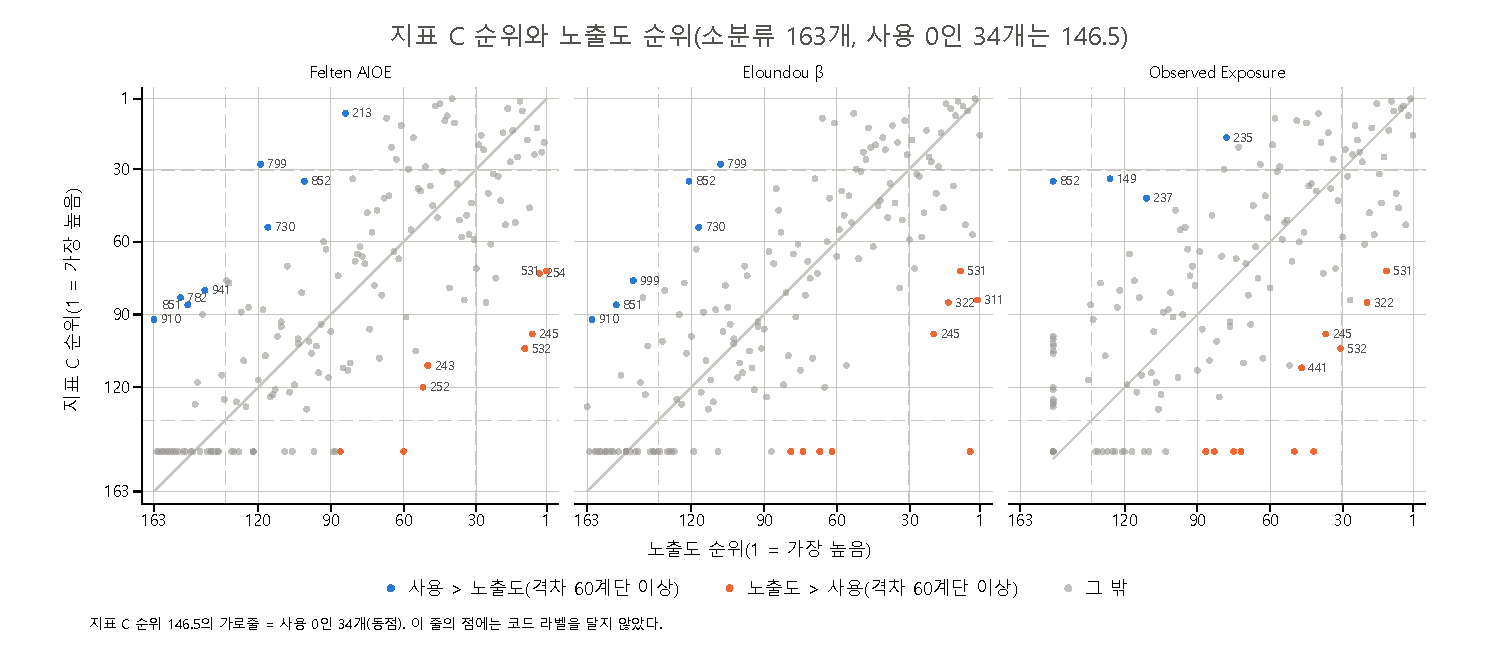
\includegraphics[width=1.0\textwidth]{../figure/35_fig_rank_scatter_C.pdf}
\caption{지표 C 순위와 노출도 순위(소분류 163개, 코드 = 격차 60계단 이상, 사용 0인 34개 제외)}\label{fig:scatter}
\end{figure}


\subsection{상위$\cdot$하위 30의 겹침}

\begin{small}
\begin{longtable}{L{3.0cm}*{9}{R{1.2cm}}}
\caption{노출도 상위$\cdot$하위 30과 사용 지표 상위$\cdot$하위 30의 겹침(개)과 노출도 상위 30의 사용 순위 중앙값}\label{tab:cross}\\
\toprule
 & \multicolumn{3}{c}{지표 A} & \multicolumn{3}{c}{지표 B} & \multicolumn{3}{c}{지표 C} \\
노출도 & 상위 & 하위 & 순위 & 상위 & 하위 & 순위 & 상위 & 하위 & 순위 \\
\midrule
\endfirsthead
% 04_18_analysis_kor_share_exposure_rank.do가 생성. 직접 고치지 말 것.
Felten AIOE & 15 & 14 & 31.5 & 15 & 14 & 29.0 & 15 & 14 & 29.5 \\
Eloundou β & 15 & 14 & 29.0 & 15 & 13 & 30.0 & 15 & 14 & 30.5 \\
Observed Exposure & 18 & 16 & 24.5 & 17 & 17 & 24.5 & 17 & 17 & 24.5 \\

\bottomrule
\end{longtable}

\begin{longtable}{L{3.0cm}*{6}{R{1.9cm}}}
\caption{사용 지표 상위 30$\cdot$하위 30의 노출도 순위 중앙값}\label{tab:crossrev}\\
\toprule
 & \multicolumn{2}{c}{Felten} & \multicolumn{2}{c}{Eloundou $\beta$} & \multicolumn{2}{c}{Observed} \\
사용 지표 & 상위 30 & 하위 30 & 상위 30 & 하위 30 & 상위 30 & 하위 30 \\
\midrule
\endfirsthead
% 04_18_analysis_kor_share_exposure_rank.do가 생성. 직접 고치지 말 것.
지표 A & 34.0 & 98.5 & 30.5 & 96.5 & 24.5 & 102.0 \\
지표 B & 34.0 & 98.5 & 30.5 & 95.5 & 25.5 & 104.0 \\
지표 C & 34.0 & 98.5 & 30.5 & 96.5 & 25.5 & 104.0 \\

\bottomrule
\end{longtable}
\end{small}

노출도 상위 30의 절반 정도(14$\sim$18개)가 사용 상위 30에도 든다. 노출도 상위 30의 사용 순위 중앙값은 24.5$\sim$32.5위라 대체로 위쪽에 있다. 거꾸로 사용 상위 30의 노출도 순위 중앙값은 24.5$\sim$34.0위, 사용 하위 목록(사용 0인 34개)은 130.0$\sim$139.5위다. 사용 0인 직업은 노출도도 대체로 낮다. 겹침 수와 순위 중앙값으로는 Observed Exposure가 사용 순위와 가장 잘 맞는다(순위상관은 세 노출도가 0.73$\sim$0.75로 비슷하다). Observed Exposure 자체가 Claude 업무 사용 기록으로 만든 지표라는 점이 영향을 준 것으로 보인다.

\subsection{지표 C 상위 10의 노출도 순위}

\begin{small}
\begin{longtable}{R{0.4cm}L{5.4cm}R{1.3cm}R{2.2cm}R{2.4cm}R{2.4cm}}
\caption{지표 C 상위 10 소분류의 노출도 값(괄호는 163개 안 순위)}\label{tab:topc}\\
\toprule
 & 소분류 & C(\%) & Felten & Eloundou $\beta$ & Observed \\
\midrule
\endfirsthead
% 04_18_analysis_kor_share_exposure_rank.do가 생성. 직접 고치지 말 것.
1 & 222 컴퓨터 시스템 및 소프트웨어 전문가 & 11.56 & 0.90 (40) & 0.81 (3) & 0.402 (2) \\
2 & 291 작가 및 언론 관련 전문가 & 11.08 & 1.24 (12) & 0.71 (9) & 0.276 (10) \\
3 & 372 비서 및 사무 지원 종사자 & 5.81 & 0.66 (45) & 0.63 (14) & 0.228 (16) \\
4 & 225 정보 시스템 및 웹 운영자 & 5.13 & 0.62 (47) & 0.72 (7) & 0.353 (5) \\
5 & 283 상품 기획‧홍보 및 조사 전문가 & 5.06 & 1.13 (17) & 0.65 (12) & 0.351 (6) \\
6 & 332 통계‧데이터 관련 사무원 & 4.20 & 1.25 (11) & 0.79 (5) & 0.299 (9) \\
7 & 213 생명 및 자연과학 관련 시험원 & 3.51 & -0.07 (83) & 0.44 (52) & 0.129 (40) \\
8 & 223 네트워크 및 정보 보안 전문가 & 3.51 & 0.82 (42) & 0.70 (10) & 0.388 (3) \\
9 & 293 연극‧영화 및 영상 전문가 & 2.91 & 0.32 (66) & 0.39 (64) & 0.070 (56) \\
10 & 211 생명 및 자연과학 관련 전문가 & 2.78 & 0.74 (43) & 0.49 (31) & 0.098 (48) \\

\bottomrule
\end{longtable}
\end{small}

지표 C 상위 10 중 정보 통신$\cdot$데이터 직업(222, 225, 223, 332)은 Eloundou$\cdot$Observed 순위도 10위 안팎으로 높다. 그러나 Felten 순위는 222가 40위, 225가 47위로 낮다. 213 생명 및 자연과학 관련 시험원과 293 연극$\cdot$영화 및 영상 전문가는 사용 순위는 높지만 노출도 순위는 세 지표 모두 40위 이하다.

\paragraph{노출도는 높고 사용은 적은 직업.} 노출도 셋 중 하나라도 상위 30이면서 지표 C 순위가 60위 밖인 소분류는 10개다. 그중 853 자동 조립라인 및 산업용로봇 조작원(Eloundou 5위)은 사용 0인 소분류다. 531 통신 관련 판매 종사자(Felten 1위, C 72위), 254 종교 관련 종사자(Felten 4위, C 73위), 245 영양사(Felten 7위, C 98위), 532 방문 및 노점 판매(Felten 10위, C 104위), 311 기획 및 마케팅 사무원(Eloundou 2위, C 84위), 322 운송 및 무역 사무원(Eloundou 14위, C 85위) 등이다. 판매$\cdot$상담$\cdot$교육 직업은 Felten에서만 높고, 사무 직업은 세 노출도에서 모두 높은 편이다.

\paragraph{사용은 많고 노출도는 낮은 직업.} 지표 C 상위 30이면서 노출도 셋 모두 40위 밖인 소분류는 293 연극$\cdot$영화 및 영상 전문가(C 9위), 235 기계$\cdot$로봇공학 기술자(17위), 239 기타 공학 전문가(21위), 799 기타 기능 관련 종사자(28위), 236 소방$\cdot$방재$\cdot$산업안전 기술자(30위)다. 이 직업들의 사용이 많은 이유는 연계표로 들어온 SOC 구성(paper 26)을 함께 봐야 한다.

\subsection{지표 C와 노출도의 사분면}

\textcite{cheon-2025-ai-exposure-vs-ai-adoption}의 [그림 1]은 가로축에 AI 노출도, 세로축에 AI 적용도를 두고 평균값의 수평$\cdot$수직선으로 직업을 네 사분면에 나눈다. 같은 형식으로 세로축에 지표 C, 가로축에 노출도 3개를 두고 소분류 163개를 그렸다. 기준보다 큰 값이 위$\cdot$오른쪽이고, 기준과 같은 값은 아래$\cdot$왼쪽에 넣었다. 색은 그림~\ref{fig:scatter}와 같은 뜻이다(파랑 = 사용 높고 노출도 낮음, 주황 = 노출도 높고 사용 낮음, 청록 = 둘 다 높음, 회색 = 둘 다 낮음).

두 판을 그렸다. 그림~\ref{fig:quadmean}은 원 그림대로 원값과 평균선이다. 지표 C는 163개 합이 100\%인 점유율이라 평균이 100/163 $\approx$ 0.61\%로 정해져 있고, 값이 상위 직업에 몰려 있어 평균선 위에 35개만 남는다. 그래서 이 판의 사분면은 사실상 노출도의 높고 낮음만 가른다. 그림~\ref{fig:quadmed}은 이를 보완해 세로축을 로그로 바꾸고 기준선을 163개 중앙값으로 했다. 로그축에 그릴 수 없는 사용 0인 34개는 맨 아래 ``0'' 줄에 따로 두었다.

\begin{small}
\begin{longtable}{L{1.3cm}L{3.0cm}R{1.3cm}R{1.4cm}R{1.3cm}R{1.3cm}R{1.3cm}R{1.4cm}R{1.8cm}}
\caption{사분면별 소분류 수(소분류 163개)}\label{tab:quad}\\
\toprule
기준선 & 노출도 & 노출도 기준값 & C 기준값(\%) & 오른쪽 위 & 왼쪽 위 & 왼쪽 아래 & 오른쪽 아래 & 오른쪽 아래 중 사용 0 \\
\midrule
\endfirsthead
평균 & Felten AIOE & -0.004 & 0.613 & 32 & 3 & 79 & 49 & 1 \\
평균 & Eloundou \(\beta\) &  0.327 & 0.613 & 33 & 2 & 86 & 42 & 4 \\
평균 & Observed Exposure &  0.077 & 0.613 & 26 & 9 & 98 & 30 & 2 \\
중앙값 & Felten AIOE & -0.025 & 0.069 & 69 & 12 & 69 & 13 & 1 \\
중앙값 & Eloundou \(\beta\) &  0.295 & 0.069 & 66 & 15 & 66 & 16 & 5 \\
중앙값 & Observed Exposure &  0.031 & 0.069 & 64 & 17 & 64 & 18 & 4 \\

\bottomrule
\end{longtable}
\end{small}
\noindent 오른쪽 위 = 노출도와 지표 C 모두 기준보다 큼, 왼쪽 위 = 지표 C만 큼, 왼쪽 아래 = 둘 다 기준 이하, 오른쪽 아래 = 노출도만 큼.

\begin{itemize}[leftmargin=*]
  \item \textbf{평균선 판}: 평균선 위의 35개는 대부분 오른쪽 위(26$\sim$33개)다. 왼쪽 위는 2$\sim$9개뿐이고(Felten에서는 213 생명 및 자연과학 관련 시험원 등 3개), 노출도가 평균보다 높은데 지표 C가 평균에 못 미치는 오른쪽 아래가 30$\sim$49개다. 지표 C 상위 6개(222, 291, 372, 225, 283, 332)는 세 노출도 모두에서 오른쪽 위다.
  \item \textbf{중앙값$\cdot$로그축 판}: 사분면이 고르게 나뉘어, 오른쪽 위와 왼쪽 아래가 각각 64$\sim$69개, 대각선 밖 두 사분면이 각각 12$\sim$18개다. 노출도와 사용이 같은 쪽에 있는 소분류가 79$\sim$85\%다.
  \item \textbf{대각선 밖 직업}: 그림~\ref{fig:quadmed}의 라벨은 대각선 밖 사분면마다 순위 격차가 큰 4개씩이다(사용 $>$ 0). 왼쪽 위(사용 높고 노출도 낮음)는 852 냉난방 관련 설비 조작원, 799 기타 기능 관련 종사자, 730 목재$\cdot$가구 관련 기능 종사자, 213, 999 기타 서비스 관련 단순 종사자 등이고, 오른쪽 아래(노출도 높고 사용 낮음)는 245 영양사, 243 약사 및 한약사, 322 운송 및 무역 사무원, 532 방문 및 노점 판매, 311 기획 및 마케팅 사무원 등이다. paper 36에서 9개 쌍 중 7개 이상의 격차 목록에 반복해 든 소분류와 겹친다.
  \item 사용 0인 34개는 지표 C가 기준 이하라 모두 아래 사분면이고, 그중 노출도가 기준보다 높아 오른쪽 아래에 드는 것은 1$\sim$5개다(Eloundou에서는 853 자동 조립라인 및 산업용로봇 조작원 등).
  \item 원 논문의 적용도는 직업별 적용 정도이지만 지표 C는 직업 규모가 들어간 점유율이다. 큰 직업은 위쪽에 오기 쉬우므로, 사분면은 ``노출도에 비해 사용 몫이 큰 직업''으로 읽어야 한다. 원 논문은 한국고용직업분류 기준이라 사분면별 수를 직접 비교할 수 없다.
\end{itemize}

\begin{figure}[htbp]
\centering
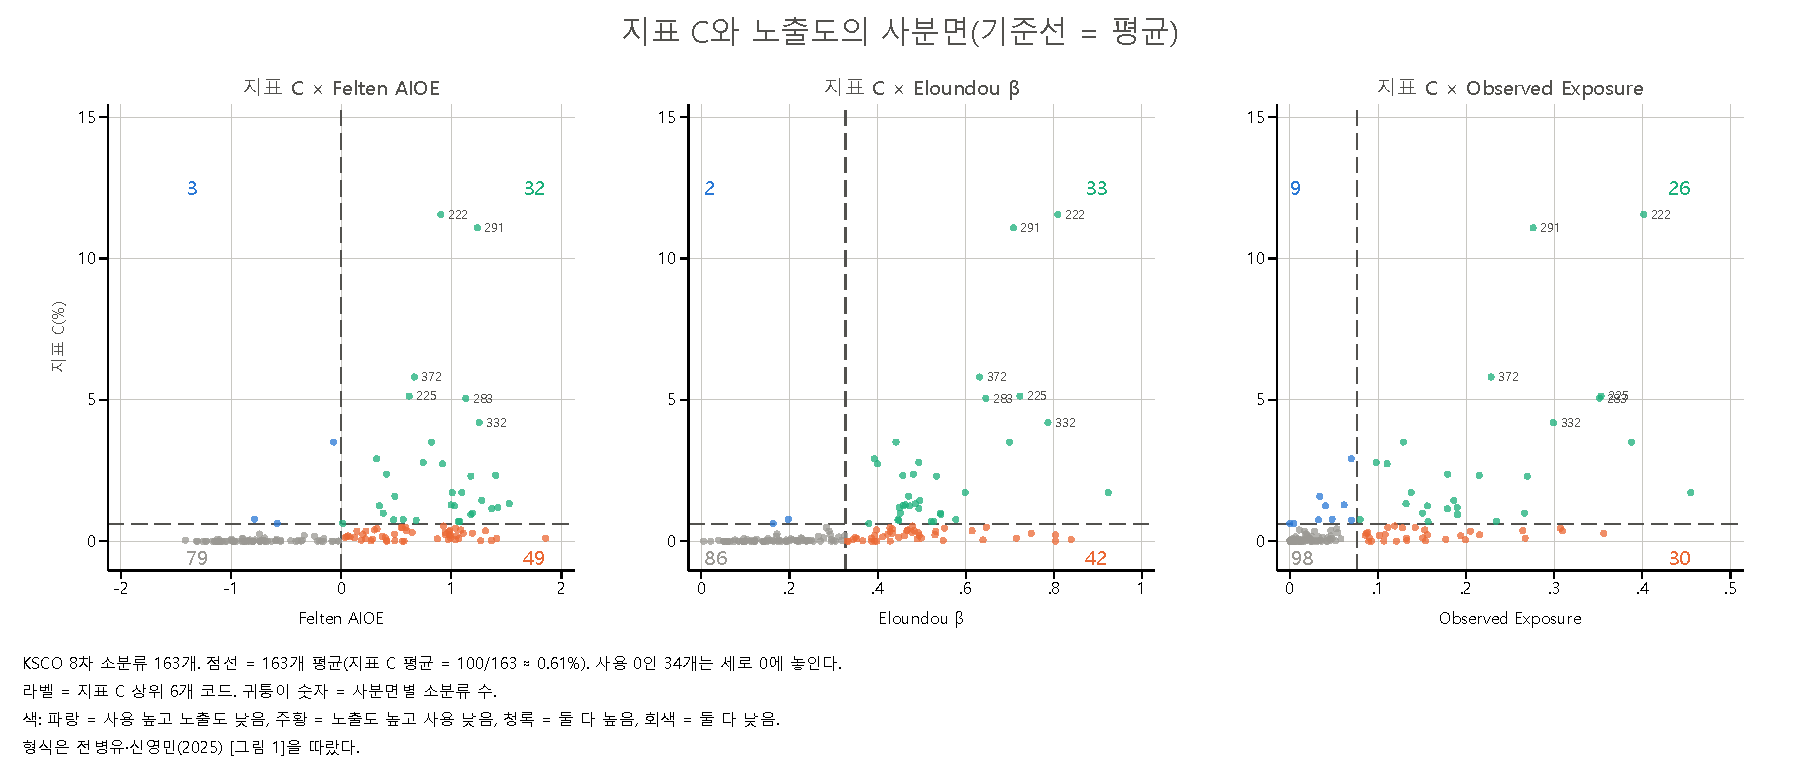
\includegraphics[width=1.0\textwidth]{../figure/35_fig_quadrant_C_mean.pdf}
\caption{지표 C와 노출도의 사분면(원값, 기준선 = 평균; 전병유$\cdot$신영민(2025) [그림 1] 형식)}\label{fig:quadmean}
\end{figure}

\begin{figure}[htbp]
\centering
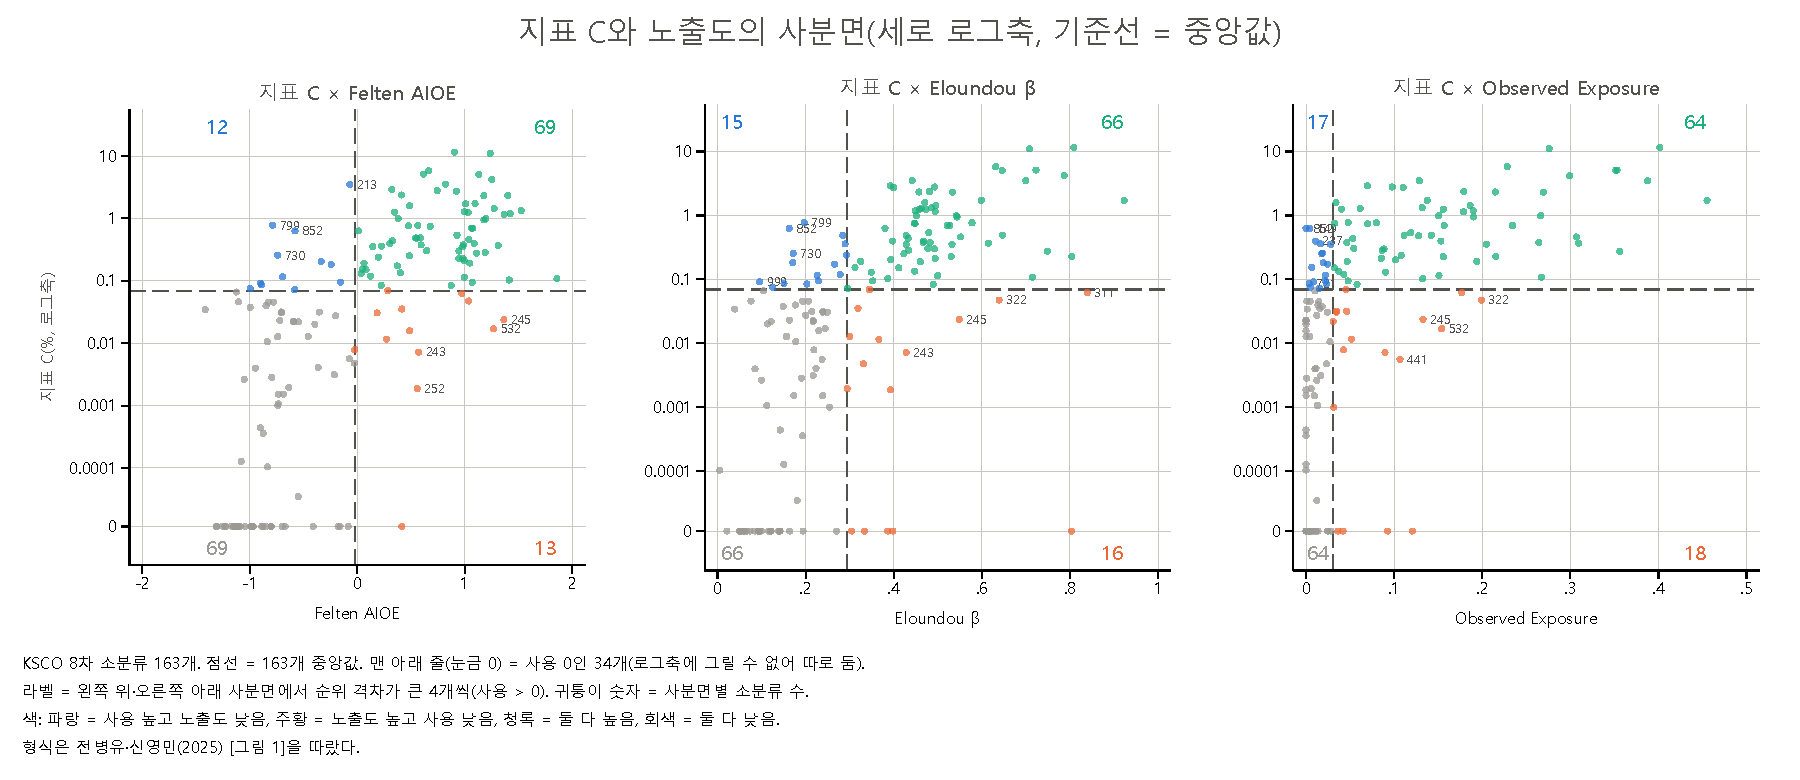
\includegraphics[width=1.0\textwidth]{../figure/35_fig_quadrant_C_med.pdf}
\caption{지표 C와 노출도의 사분면(세로 로그축, 기준선 = 중앙값)}\label{fig:quadmed}
\end{figure}

\section{읽을 때 유의사항}

\begin{longtable}{L{12.5cm}R{2.5cm}}
\caption{점검 수치}\label{tab:notes}\\
\toprule
항목 & 값 \\
\midrule
\endfirsthead
% 04_18_analysis_kor_share_exposure_rank.do가 생성. 직접 고치지 말 것.
비교 소분류 수 / 그중 사용 0(지표 A·B·C = 0, 평균 순위 동점) & 163 / 34 \\
Observed Exposure가 0인 소분류 수(평균 순위 동점) & 28 \\
Felten AIOE가 음수인 소분류 수 & 82 \\
Eloundou $\beta$의 서로 다른 값 수 & 157 \\
한 달만 공개된 소분류 수 / 그중 지표 C 하위 목록에 든 수 & 7 / 0 \\
상위 / 하위 목록 크기(A, B, C, Felten, Eloundou, OE; 경계 동점 포함) & 30/34, 30/34, 30/34, 30/30, 30/30, 30/30 \\

\bottomrule
\end{longtable}

\begin{enumerate}[leftmargin=*]
  \item \textbf{Observed Exposure가 0인 28개는 동점이다.} 값이 0인 소분류 28개(사용이 있는 13개: 252, 263, 422, 453, 611, 620, 630, 710, 852, 871, 881, 882, 952와 사용 0인 15개)는 모두 149.5위다. 852 냉난방 관련 설비 조작원은 Observed Exposure가 0인데 지표 C는 35위다.
  \item \textbf{지표 C 하위 목록은 사용 0인 34개다.} 이들의 0은 실제 사용이 없다는 뜻이라기보다 연결된 SOC의 한국 비중이 공개되지 않았다는 뜻이다. 한 달만 공개된 소분류 7개는 그 바로 위(118$\sim$129위)에 있고, 비공개 달을 0으로 두고 평균해 값이 절반이 됐다(paper 27). 하위권의 사용 순위에는 공개 범위의 영향이 섞여 있다.
  \item \textbf{점유율은 규모가 들어간 값이고 노출도는 강도다.} 큰 직업은 점유율 순위가 올라가기 쉽다. 규모를 뺀 비교는 상대 활용도 RU1$\cdot$RU2(paper 25, 32)나 노출도 기반 점유율(paper 28, 33)로 본다.
  \item \textbf{두 쪽 모두 SOC 값을 연계표로 옮긴 것이다.} 사용은 \texttt{w\_alloc}으로 배분하고, 노출도는 \texttt{w\_mean}으로 평균했다(paper 21, 23). 연계 경로가 한 SOC에 쏠린 소분류는 그 SOC의 값에 따라 순위가 크게 움직인다.
  \item \textbf{순위 차이 자체의 분석은 다른 paper에 있다.} 순위 격차의 회귀 분석과 강건성은 paper 29, 분산$\cdot$쏠림의 비교는 paper 33이다. 이 파일은 목록을 직접 확인하기 위한 표다.
\end{enumerate}

\section{산출 파일}

\begin{itemize}[leftmargin=*]
  \item 코드: \texttt{code/04\_18\_analysis\_kor\_share\_exposure\_rank.do}(Stata 17, \texttt{00\_master.do}에 포함). 입력은 \texttt{data/proc/merged/kor\_ai\_usage\_ksco3.dta}(\texttt{03\_05}).
  \item 엑셀: \texttt{results/table/35\_kor\_share\_exposure\_rank.xlsx}(시트 7개).
  \item 이 노트의 표: \texttt{results/table/35\_spearman.tex}, \texttt{35\_cross.tex}, \texttt{35\_cross\_rev.tex}, \texttt{35\_topC10.tex}, \texttt{35\_notes.tex}.
  \item 그림: \texttt{results/figure/35\_fig\_rank\_scatter\_C.\{pdf,png\}}, \texttt{35\_fig\_quadrant\_C\_mean.\{pdf,png\}}, \texttt{35\_fig\_quadrant\_C\_med.\{pdf,png\}}(\texttt{code/04\_20\_analysis\_kor\_share\_figures.do}). 사분면 표 \texttt{results/table/35\_quadrant.tex}도 같은 do 파일이 만든다.
\end{itemize}

\printbibliography[title={참고문헌}]

\end{document}
